\section{Spletni portali za učenje programiranja}
\label{sec:SPUP}

Spletne portale za učenje programiranja (\textbf{SPUP}) bomo
predstavili in spoznali tako, da bomo najprej pregledali, kaj so bili
glavni razlogi, da so se pojavili. Spletni portali za učenje
programiranja, v nadaljevanju \textbf{SPUP}, so nastali takoj po
razmahu interneta v začetku novega tisočletja. Najprej so nastali na
univerzah. Zanima pa nas, kaj so glavni razlogi za nastanek SPUP.  Poleg
tehnoloških zmožnosti IKT za nastanek spletnega portala nas zanimajo
predvsem težave, ki so jih skušali premostiti z uporabo SPUP.

Spletni portali so nastali na različnih univerzah, ogledali si bomo
spletni portal, ki je nastal na \emph{Odprti univerzi v Hong
  Kongu} (\textbf{OUHK}), na \emph{Univerzi Strathclyde v Veliki
  Britaniji} (\textbf{USVB}) in \emph{Queensland University of
  Technology, Australia} (\textbf {QUTA}).

Zanimali nas bodo predmeti, ki veljajo za začetne pri poučevanju
računalniške znanosti in programiranja. \textbf{Novinci}, kot jih bomo
imenovali, so študenti, ki se šele začnejo učiti programiranja. V
diplomskem delu nas zanimajo le učenci osnovnih šol in dijaki
srednjih, vendar se oni prav tako šele srečujejo s programiranjem,
podobno kot študentje, in jih bomo zato vse poimenovali kot
\textbf{novince}.

%%OPOMBA: To trdim brez citata.
Kot je razvidno iz literature, bomo lahko sklepali na nekatere skupne
značilnosti vseh novincev, ne glede na težavnostno stopnjo, na kateri
se nahajajo, saj je programiranje veščina, ki ni dana naravno in se je
mora vsak priučiti.

%Kaj je spletni portal?

%Spletni sistem omogoča študentom in mentorjem spletno okolje za učenje
%programiran.

%Kako opredelimo kaj je to (ang. Course) ali je to en predmet, ali
%skupek predmetov.

\subsection{Razlogi za nastanek spletnih portalov}
\label{sec:razlogi_za_nastanek_SPUP}

Na Odprti univerzi v Hong Kongu (\textbf{OUHK}) ponujajo tri
računalniške sklope različnih težavnosti za dodiplomske
programe. Imajo zelo veliko populacijo študentov, ki se učijo
programiranja. Avtorji članka \cite{ITaLCP_DistanceEdu}
ugotavljajo, da je proces učenja programiranja kompleksen in zahteva
veliko vaje. Izkaže se, da praktični
del igra poglavitno vlogo v učnem procesu.

Glavna težava, s katero se srečujejo na \textbf{OUHK}, je ta, da se
število študentov, ki se vpišejo v smeri računalništva,
povečuje. Povečanje študentov pomeni manj časa za mentorstvo za
posameznega študenta.

Da bi študentje lahko normalno sledili pouku na daljavo, si morajo
doma urediti delovno okolje, kjer lahko programirajo. Študenti,
dobijo vso potrebno učno literaturo in tudi programsko opremo, ki
predstavlja \textbf{prevajalnik} in \textbf{razvojno okolje}. Izkaže se,
da imajo številni težavo nastaviti in se spoznati z integriranim
razvojnim okoljem (\emph{ang. Integrated Development Environment
  (\textbf{IDE})}) \cite{ITaLCP_DistanceEdu}.

Težave pri izobraževanju na daljavo se pojavijo tudi v
komunikaciji. Študent, ki se izobražuje od doma in naleti na neko
težavo, ki je ne zna sam rešiti, nima dostopa do svojih kolegov ali
mentorjev. Do mentorjev lahko dostopa le preko telefonskih klicev ali
elektronske pošte. Če pogledamo še s strani mentorjev, imajo ti težavo
s spremljanjem napredka velikega števila študentov.

%%Tu pride uvod z naslednjega članka!

Naslednji članek, ki so ga sestavili avtorji z \emph{Univerze
  Strathclyde iz Velike Britanije} (\textbf{USVB}), se ukvarja z
raziskovanjem vpliva nove strategije kognitivnega pristopa k
poučevanju programiranja, ki spreminja mentalni model študentom tako,
da v njih ustvari konflikt. V ta namen je bilo razvito tudi spletno
okolje, ki implementira uporabo nove kognitivne strategije
\cite{mentalModels}.

%kaj točno je mentalni model in ali je to pravi prevod

Kot pravijo avtorji v članku, s hitrim razvojem IKT narašča tudi
potreba po sposobnih programerjih in učenje programiranja postaja
globalna skrb. V prvem letu pri predmetih programiranja študenti
obvladajo naloge programiranja dosti slabše, kot bi to
pričakovali. Slaba uspešnost se pozna predvsem pri tem, da se mnogi
izpišejo s smeri računalništva, takih je kar od 30 do 50 \%. Kot
avtorji poudarjajo in povzemajo po drugih študijah, so za to v glavnem
krive težave pri reševanju problemskih nalog, ki nastopajo v
programiranju. Nekatere druge študija vidijo krivca za neuspeh tudi v
napačnem razumevanju ključnih konceptov pri programiranju, ki so lahko
posledično krivi za težave pri reševanju problemov. Tradicionalni učni
pristop je za učenje programiranja manj zanesljiv, da bi zagotovil
pravilnost v razvoju mentalnih modelov o konceptih
programiranja. Študije kažejo, da študenti po enem letu predmeta
programiranja še vedno nimajo pravih mentalnih modelov o osnovnih
programskih konceptih.

Na univerzi QUTA se pri začetnih predmetih programiranja srečujejo s
podobnimi težavami kot na OUHK in USVB.

\begin{enumerate}
\tightlist
\item Namestitev in nastavitve okolja za programiranje.
\item Uporaba urejevalnika besedil.
\item Razumevanje programskih vprašanj in uporabe sintakse jezika pri
  pisanju programske kode.
\item Razumevanje napak prevajalnika.
\item Razhroščevanje.
\end{enumerate}

Ugotavljajo, da je pri danih vajah programiranja pomembno, da ob
težavah novinci dobijo čimprajšni odziv mentorja. V velikih razredih
se to izkaže za zelo zahtevno. Tudi začetniki, ki uspešno premagajo
začetne ovire in se lotijo takojšnjega programiranja, imajo zelo slabo
napisano in konstruirano programsko kodo. Pomagati študentom pisati
kakovostno programsko kodo je prav tako časovno zelo zahtevno. Težave
programiranja se stopnjujejo, ko se za učenje progremiranja uporabljajo
OO programski jeziki, saj ti zahtevajo visoko stopnjo
abstraktnega razumevanja programskih konceptov. Za izdelavo spletnega
portala za učenje programiranja so na QUTA bili pomembni naslednji
cilji \cite{thesisAWebP}.

\begin{itemize}
\item Omogočiti lažji začetek pri učenju programiranja s pogostim
  odzivom mentorjev na težave novincev. S pomočjo ob pravem času
  spremenimo odnos novincev do programiranja.
\item Izboljšati uspeh začetnih predmetov programiranja.
\item Pomoč mentorjem pri učenju in administraciji predmetov
  programiranja.
\end{itemize}

\subsection{Primeri implementacije in sistemska arhitektura}
\label{sec:sistemska_arhitektura_All}

Zanimalo nas je tudi, kakšna je morebitna sistemska arhitektura takega
spletnega portala, zato si pomagamo s primerom arhitekture, ki so ga
izdelali na \textbf{OUHK}.  V nadaljevanju govorimo o
\emph{aktivnostih}, ki jih mora študent opraviti, to so naloge,
programske rešitve na zastavljene probleme. Študenti na \textbf{OUHK}
se učijo programiranja v programskem jeziku \textbf{Java}.

Kot prikazuje slika \ref{fig:OUHK_cmsArch}, je sistem urejanja vsebine
(\emph{ang. Contetnt Managment System (\textbf{CMS})}), teče na
spletnem strežniku \emph{\href{http://www.apache.org/}{Apache}} z
\emph{\href{https://www.mysql.com/}{MySQL}} podatkovno bazo. Sistem je
narejen iz štirih podmodulov, ki so napisani v skriptnem jeziku
\emph{\href{http://php.net/}{PHP}}.

\begin{figure}[htb!] \centering
  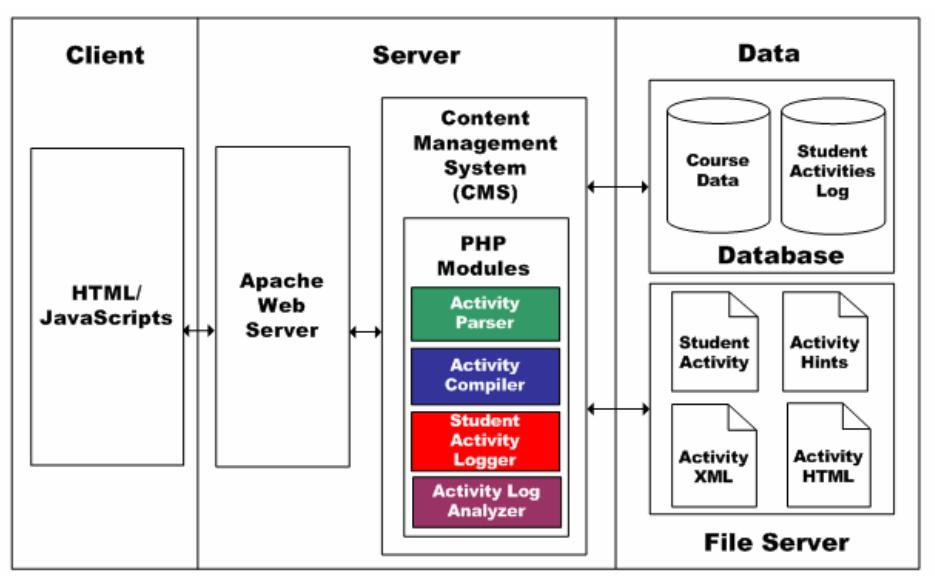
\includegraphics[width=0.9\linewidth, keepaspectratio =
1]{./images/SystemArch01_OUHK_DistanceEdu.jpg}
  \caption{Sistemska arhitektura spletnega portala za učenje
    programiranja, kot so jo naredili na OUHK \cite{ITaLCP_DistanceEdu}.}
  \label{fig:OUHK_cmsArch}
\end{figure}

Ti moduli so naslednji: zajem aktivnosti, prevajalnik aktivnosti,
dnevnik študentove aktivnosti in analizator dnevnikov aktivnosti. Samo
delovanje je naslednje: ko odjemalec pošlje zahtevo za neko aktivnost,
se ta naslovi strežniku, ki poišče programsko aktivnost. Z modulom
\emph{zajema aktivnosti} strežnik zajame aktivnost, ki je zapisana v
obliki \textbf{XML}, in naloži vse potrebne datoteke. Zajem aktivnosti
prav tako naloži študentovo predhodno delo, ki je shranjeno v datoteki
aktivnosti. Ko se vse zajame in naloži, se vsebina pošlje v obliki
\textbf{HTML} nazaj h klientu.

Strežnik omogoča tudi prevajanje aktivnosti. Ko strežnik dobi prošnjo
za prevajanje programske kode, se ta prevede, če v njej ni
sintaktičnih napak, in se ustvari datoteka \textbf{JAR}, ki jo študent
lahko prenese s strežnika. Če so v programu napake, se ustvari dnevnik
napake v trenutni aktivnosti, prav tako se napaka izpiše na zaslonu
študenta. Vsako aktivnost zajame dnevnik študentove aktivnosti in jo shrani v
podatkovno bazo. Z analizatorjem dnevnika študentove aktivnosti
mentorji dobijo vpogled v delo študenta in njegovega napredka.

\subsection{Pregled delovanja in interakcija s SPUP}
\label{sec:pregled_delovanja_in_interakcija}

Opišimo, kako so si zamislili interakcijo med študentom in mentorjev s
spletnim sistemom na \textbf{OUHK}. Diagram prikazuje slika
\ref{fig:OUHK_workFlow}. Spletni sistem omogoča študentom in mentorjem
spletno okolje za učenje programiranja. Mentorji na spletni portal
naložijo snov preko spletnega brskalnika. Mentor lahko naloži datoteke z
opisom aktivnosti. Ta datoteka vsebuje osnovne opise in informacije o
aktivnostih. Posebej naloži še datoteko, v kateri je predloga za
aktivnost. V to predlogo študent rešuje zadano nalogo. V posebno
datoteko je naložen tudi namig, ta je študentu v pomoč in ponuja
primer izpisa programa.
%Potreben prevod slike!
\begin{figure}[htb!] \centering
  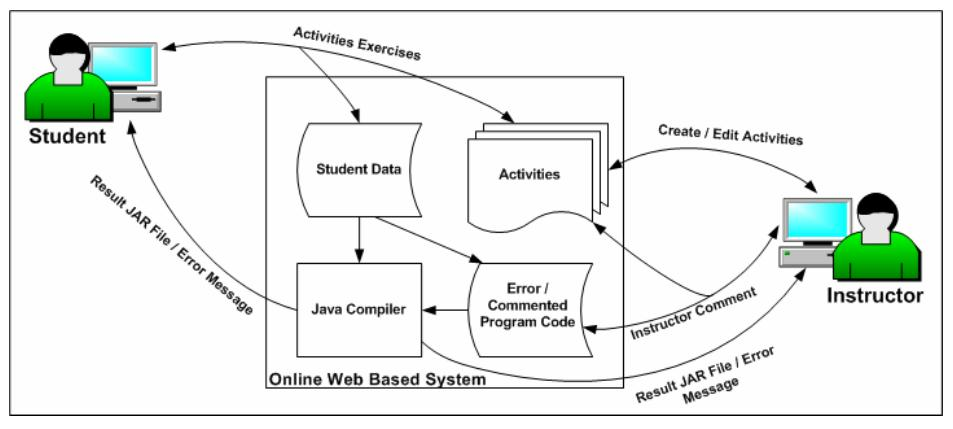
\includegraphics[width=0.9\linewidth, keepaspectratio =
1]{./images/SystemArch02_OUHK_DistanceEdu.jpg}
\caption{Prikaz interakcije med študentom in mentorjem s spletnim
  portalom \cite{ITaLCP_DistanceEdu}.}
  \label{fig:OUHK_workFlow}
\end{figure}

Študent lahko pregleduje vse aktivnosti in si naloži katero koli izmed
njih. Omogočeno ima, da program prevede na strežniku, ko prevajalnik
naleti na napake, strežnik vrne napako na spletno stran. Če študent
naleti na težavo, ki je povezana z reševanjem aktivnosti, lahko pošlje
prošnjo za pomoč svojemu mentorju. Ko se mentor prijavi v sistem, ima
vpogled v napako in na začasno delovno datoteko študenta, mentor lahko
zaganja prevajalnik na tem začasnem projektu študenta. Ko mentor
popravi programsko napako, odgovori študentu in poda komentar na
programsko kodo študenta. Študent ima vpogled v komentarje in
predloge, ki jih je posredoval mentor \cite{ITaLCP_DistanceEdu}.

%%NJihova diskusija, zaključek in nadaljnjo delo.

Na univerzi v US \cite{mentalModels} je okrog strategije kognitivnega
konflikta nastalo spletno okolje, ki naj bi izboljšalo mentalne modele
ključnih programskih konceptov. Učni model je sestavljen iz štirih
korakov:

\begin{itemize}
\item \textbf{Predhodni korak:} mentor razišče, kakšni so predhodni
 mentalni modeli študentov, in identificira neprimerne.
\item \textbf{Korak kognitivnega konflikta:} v študentovi predstavi
  mora sprožiti tak dogodek, ki v študentu izzove neskladje z njegovo
  predhodno predstavo in s tem se študenta potisne v konfliktno
  situacijo.
\item \textbf{Korak konstruiranja modela:} vizualizacija študentu
  pomaga ustvariti pravo mentalno predstavo.
\item \textbf{Korak aplikacije:} študent mora rešiti programsko
  nalogo z na novo ustvarjeno mentalno predstavo.
\end{itemize}

Spletno učno okolje podpira programski jezik \textbf{Java}. Za učenje
programskih konceptov je na spletni strani vsak posamezen koncept povezan s
potjo, ki predstavlja načrt potovanja. Poti konceptov se povezujejo tako, da se
ti nadgrajujejo, saj znanje določenega koncepta potrebuje neko predznanje
prejšnjega. Tako za razumevanje določevanja reference najprej potrebujemo
predznanje o spremenljivkah ali npr. preden se študenti učijo, kako se podajajo
parametri v podprograme, morajo najprej razumeti, kaj je obseg nekega
podprograma. Torej je vrstni red spoznavanja programskih konceptov pomemben. Med
potmi so gumbi, ki predstavljajo vsak koncept. Na vsakem gumbu je označen rdeč
križ, kar pomeni, da študent še ni spoznal koncepta. Ko študent opravi naloge,
povezane s posameznim konceptom, se rdeč križ spremeni v zeleno kljukico. Ko
študent vstopi v koncept, se izpiše študentova zgodovina z nalogami tega
koncepta. Vsaka naloga vsebuje tako vprašanje, ki sproži konfliktno situacijo v
mentalnem modelu študenta. Nato študenti dobijo učni material v vidni obliki. Za
vizualizacijo uporabljajo orodje
\href{https://cs.joensuu.fi/jeliot/}{\textbf{Jeliot}}, ki dinamično upodablja
izvajanje javanskih programov. Za pravilnost razumevanje mentalnega modela mora
študent odgovoriti na dodatna vprašanja. Če študentovi odgovori niso v skladu s
podanim mentalnim modelom, dobi študent povratno informacijo o nepravilnem
odgovoru. Naslednji korak je ta, da mora študent zagnati vizualizacijo dela
programske kode, ki si ga je prej moral predstavljati. Tako ima možnost, da
zazna nepravilnost v svojem mišljenju in tako lahko gradi na pravilnem konceptu
\cite{mentalModels}.

%% QUTA
V preteklosti je bilo razvitih mnogo orodij, ki so nastala ravno zaradi
raziskovanja učenja programiranja, vendar mnoga od teh zahtevajo, da
študenti pišejo celotne programe od začetka do konca. Spletni portal
v primeru QUTA uči programiranja v programskem jeziku Java in ima
 naslednje zmožnosti \cite{thesisAWebP}.

\begin{enumerate}
\tightlist
\item Spletni portal za programiranja, ki omogoča naloge tipa ``zapolni
   prazna mesta''. % pri "zapolni prazna mesta se ti izpiše Ž namesto z!
\item Ogrodje za analizo, ki preverja kakovost in pravilnost, nalog
   tipa "zapolni prazna mesta".
\item  Samodejni sistem za dajanje povratnih informacij, ki sporoča
   prilagojena sporočila prevajalnika in formalni odziv študentom in
   njihovim mentorjem. Poročilo vsebuje kakovost napisanega programa,
   strukturo in pravilnost glede na programsko analizo.
\end{enumerate}

\subsection{Rezultati izvedenih rešitev SPUP}
\label{sec:rezultati_izvedenih_rešitev}

Večina študentov smeri računalništva na OUHK nima predhodnih izkušenj
v programiranju s programskim jezikom \textbf{Java}. Sistem se
uporablja kot spletno okolje za učenje programiranja. Študentom je s
tem dana množica aktivnosti oz. nalog, ki jih morajo sami uspešno
opraviti. To lahko počnejo kadarkoli in kjerkoli. Študentom ni
treba nastavljati programskega okolja, študenti vse programe, ki
jih napišejo, lahko takoj prevedejo in jih zaganjajo na svojih
računalnikih. Uporaba spletnega portala je pokazala, da so študentje
oddali 100 \% programskih nalog, napisanih v Javi. Kar kaže na to, da so
študentje samozavestno reševali naloge in jih oddajali. Pred uporabo
spletnega portala je oddaja nalog bila 80 \%.

Kot pravijo avtorji članka in portala \cite{ITaLCP_DistanceEdu}, je to
šele začetek uporabe spletnega portala, ki nudi osnovno
funkcionalnost. V nadaljevanju nameravajo dodati še inteligentni
sistem, ki bo nadzoroval napredek študentov.

Za izboljšanje mentalnih modelov, ki avtorji predlagajo konstruktivno
naravnan učni model, ki vključuje strategijo kognitivnega konflikta in
vizualizacijo programov. Zgodnje preizkušanje strategije kognitivnega
konflikta pokažejo, da so študenti bolj zavzeti za učni material in jih
motivira tako, da si prej ustvarijo pravilno mentalno predstavo
\cite{mentalModels}.

Tudi začetniki, ki uspešno premagajo začetne ovire in se lotijo
takojšnjega programiranja, imajo zelo slabo napisano in konstruirano
programsko kodo. Pomagati novincem pisati kakovostno programsko kodo
je časovno zelo zahtevno opravilo.

% Torej je pomembno v katerih programskih jezikih se začnemo učiti
% programiranja? Zakaj sta zato primerna? -> Scratch in Python?  Kje
% je določeno na državnem nivoju da se učit ravno ta dva programska
% jezika

Rezultat dela avtorjev spletnega portala QUTA gre še nekoliko naprej
od OUHK in v njihov spletni portal vgradijo odziv spletnega portala,
ki javlja o pravilnosti programa in o kakovosti. Ogrodje
\emph{(ang. framework)} za analizo programske kode vsebuje naslednje
komponente \cite{thesisAWebP}:

\begin{itemize}
\tightlist
\item
  sintaktično ali semantično opozarjanje na napake ali napake
  prevajalnika,
\item
  odziv na kakovost in pravilnost programske kode,
\item
  formalni odziv učitelja oz. komunikacija med učiteljem in učencem.
\end{itemize}

\subsection{Značilnosti SPUP}
\label{sec:značilnosti_spup}

Ena od osnovnih in glavnih komponent pri vseh SPUP je orodje, ki
omogoča pisanje in preizkušanje programske kode. Poimenujemo jo lahko
kot \textbf{spletna aplikacija za programiranje (SAZP)}. Njene
glavne značilnosti so naslednje:

\begin{itemize}
  \item \textbf{urejevalnik besedil}, ki ima lahko osnovne funkcije ali tudi
  zahtevne, ki so značilne za \textbf{IRO};
\item omogočen je zagon napisanega progama z vhodnimi in izhodnimi
  podatki;
\item omogočena je \textbf{povratna informacija}:
  \begin{itemize}
    \tightlist
  \item \textbf{sintaktičnih napak}, ki ju vrne prevajalnik ali tolmač;
  \item \textbf{semantičnih napak}, ki preverjajo želen rezultat napisanega
    programa oz. pravilno rešitev.
  \end{itemize}
\end{itemize}

Iz pregleda SPUP, ki so nastali na univerzah, smo se lahko poučili, kaj
so nekatere značilnosti spletnih portalov. Strnimo te značilnosti, saj
jih bomo pozneje uporabili pri iskanju, kategoriziranju in
vrednotenju. Spletni portal vsebuje naslednje elemente:

\begin{itemize}
\tightlist
\item razdelano vsebino z nalogami oz. aktivnostmi,
\item \textbf{spletno aplikacijo za pisanje programske kode},
\item omogočena je komunikacija med mentorjem in novincem,
\item omogočen je pregled nad napredkom novincev oz. tako imenovan
  \emph{nadzor nad razredom}.
\end{itemize}


%%% Local Variables:
%%% mode: latex
%%% TeX-master: "../diploma"
%%% End:
